\subsection{Bode Plots}
    \subsubsection{Decibel scale}
        $z_{\text{dB}} = 20 * \log_{10}(z_{\text{decimal}})$\\
        Important values on decibel scale:
        \begin{tabu}{X X}
            
        \end{tabu}
    
    \subsubsection{Drawing the Bode plot}
        \begin{tabu}{| X | X | X |}
            \hline
            pole / zero type & change in magnitude & phase shift\\
            \hline \hline
            BIBO stable pole or integrator 1/s & -20dB/dec & $-90^{\circ}$\\
            \hline
            BIBO unstable pole & -20dB/dec & $+90^{\circ}$\\
            \hline
            minimum phase zero or differentiator s & +20dB/dec & $+90^{\circ}$\\
            \hline
            non-minimum phase zero & +20dB/dec & $-90^{\circ}$\\
            \hline
        \end{tabu}
        \begin{itemize}
            \item position of complex poles / zeros: $\omega_n = \sqrt{\sigma^2 + \omega^2}$
            \item Slope of magnitude changes at pole / zero
            \item angle changes within a decade before and afer the pole/zero
            \item For $G(s)$ with incoming slope: calculate $|G(j \omega)|$ for $\omega = 1$
        \end{itemize}

    \subsubsection{Adding Bode Plots}
        Bode plot of $T(s) = k_1 \cdot T_1(s) + k_2 \cdot T_2(s)$ with given bode plots of $T_1(s)$ and $T_2(s)$:
        Bode plot of $T(s)$ is the addition of the Bode plots of $T_1(s)$ and $T_2(s)$ with respect to $k_1, k_2$

    \subsubsection{Inverted Transfer Function}
        Bode plot $T^{-1}(s)$ is the Bode plot $T(s)$ reflected about horizontal axis

    \subsubsection{Stability in Bode Plots}
        \begin{minipage}{0.64 \linewidth}
            \titel{crossover frequency, phase and gain margin}
                Bode plot of open loop system $\rightarrow$ closed loop Gain and Phase margin
                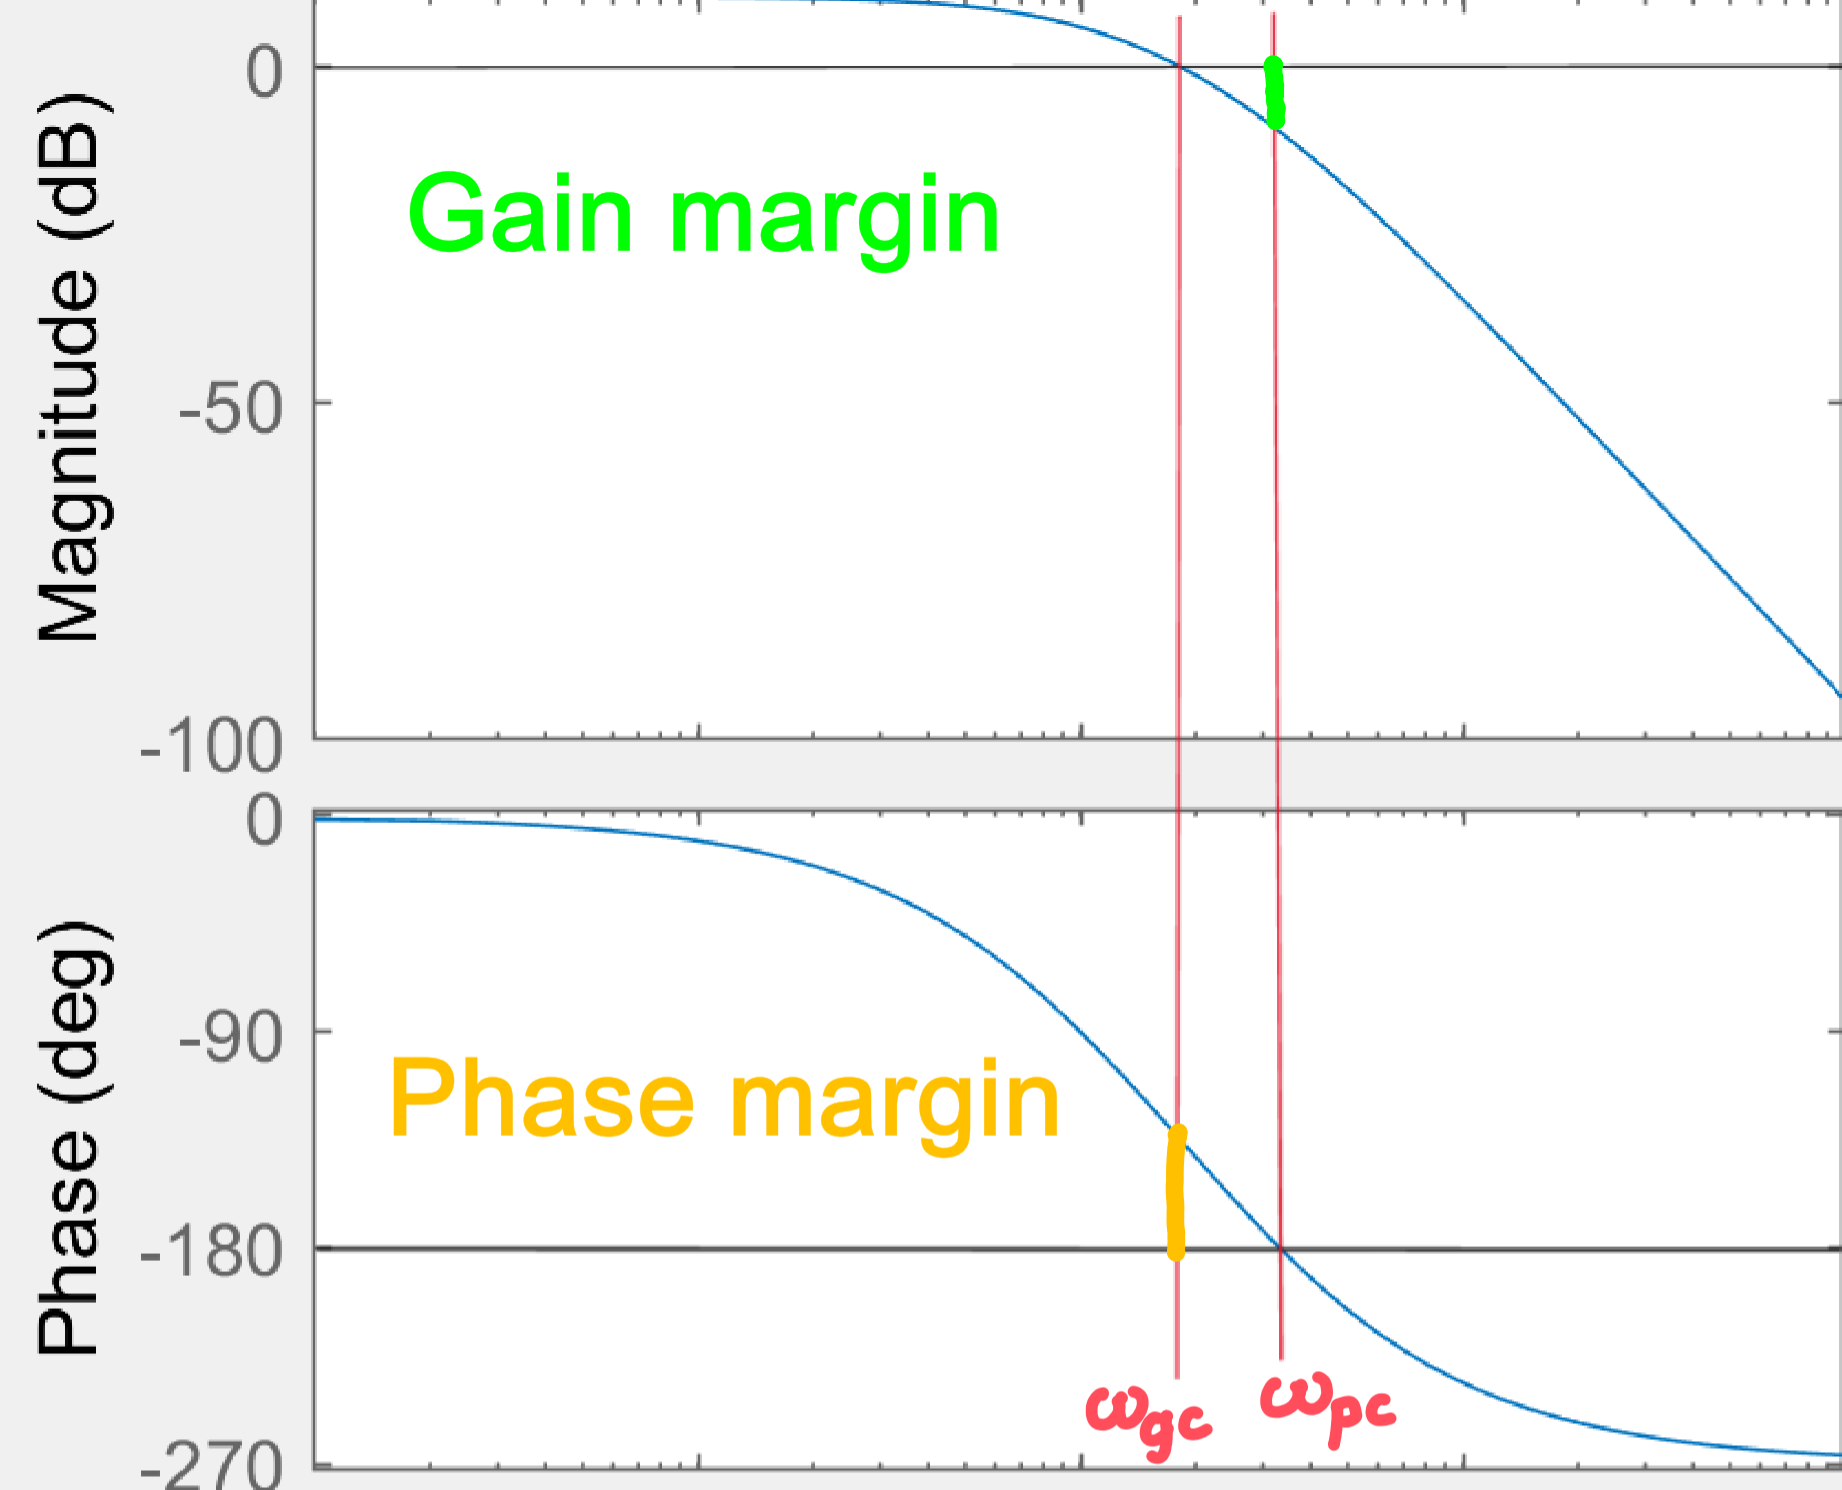
\includegraphics[width = \linewidth]{src/images/gain_phase_margin.png}
        \end{minipage}
        \begin{minipage}{0.34 \linewidth}
            \titel{stability criterion}
            For \textbf{\textit{stable}} open loop systems, the Nyquist criterion shows that the following must hold:
            \begin{align*}
                |G(j \omega_{pc})| < 0 dB\\
                \angle(G(j \omega_{pc})) > -180^{\circ}
            \end{align*}
            Crossover frequency:
            \begin{align*}
                \omega_{c} \Leftrightarrow |L(\omega_c)| = 0dB
            \end{align*}
        \end{minipage}

    

    \subsubsection{Bandwidth}
        maximum $\omega$ for which $|T(s)| > \frac{1}{\sqrt{2}}$
        Bandwidth is highest frequency a system can handle. Closed loop bandwidth $\approx$ open loop crossover frequency
        